\documentclass[11pt]{article}
%Gummi|063|=)
\title{\textbf{Operating systems -- supervision 3}}
\author{James Wood}
\usepackage{listings}
\usepackage{bold-extra}
\usepackage{xcolor}
\usepackage{amsmath}
\usepackage{enumitem}
\usepackage{tikz}
\usepackage{tabularx}
\usepackage{hyperref}
\usetikzlibrary{arrows,arrows.meta,shapes.multipart,matrix,positioning}

\lstset{
  basicstyle=\small,
  basewidth=0.5em,
  frame=single,
  breaklines=true,
  %postbreak=\raisebox{0ex}[0ex][0ex]{
  %  \ensuremath{\color{red}\hookrightarrow\space}
  %}
  language=python,
  literate=
    {<=}{{\(\leq\)}}1
    {>=}{{\(\geq\)}}1
    {&&}{{\(\wedge\)}}1
    {||}{{\(\vee\)}}1
    {->}{{\(\rightarrow\)}}1
}

\tikzset{
  treenode/.style = {align=center, inner sep=0pt, text centered,
    font=\sffamily},
  bnode/.style = {treenode, circle, white, draw=black,
    fill=black, text width=1.5em},
  rnode/.style = {treenode, circle, red, draw=red,
    text width=1.5em, very thick},
  leaf/.style = {treenode, rectangle, draw=black,
    minimum width=0.5em, minimum height=0.5em}
}

\begin{document}

\maketitle

\begin{enumerate}
\item
  \begin{enumerate}
  \item Virtual addresses mean that processes have no way of accessing memory outside their address space, the OS can change the physical location of memory without the program needing to know about it, and virtual memory can be larger than physical memory if extra storage (such as a hard disk) is used.
  \item Virtual addressing requires additional hardware to be performant. For embedded systems, the cost (by whatever metric) of the extra parts (and the time taken to translate each address) may not be worth it, since programs may have physical addresses bound at compile or load time.
  \item
    \begin{enumerate}
    \item
      In both cases, applications get access to addresses starting at 0. In the case of segmented memory, these addresses are bounded, but with paged memory, these are unbounded (though the system may crash in the event that too much memory is used). For segmented memory, there will be a simple function mapping virtual addresses to physical addresses based on what range the virtual address is in. Here is an example:

      \begin{tabular}{l|l}
        virtual address & physical address\\
        \hline
        [0..200) & [7800..8000)\\ \relax
        [200..600) & [400..800)\\ \relax
        [600..E00) & [4800..5000)\\
      \end{tabular}

      For paged memory, virtual addresses are assigned to pages, then pages are assigned to physical addresses. Here is an example state of this system:

      \begin{tabular}{l|l|l}
        virtual address & page number & physical address\\
        \hline
        [0..1000) & 5 & [24000..25000)\\ \relax
        [1000..2000) & 93 & [8000..9000)\\ \relax
        [2000..3000) & 34 & [1A000..1B000)\\
      \end{tabular}
    \item Memory allocation is easier for paged memory because finding free space requires only a lookup in the page table. With segmented memory, each PCB must be checked, and the OS has to reason about ranges.
    \item Segmented memory is more reliably quick to access, since it doesn't rely on much indirection. It also doesn't require as much hardware support, since paging is usually supplemented with a TLB.
    \end{enumerate}
  \end{enumerate}
\item
  \begin{enumerate}
  \item Internal fragmentation occurs when a process has been allocated more memory than it needs. This could occur because of a memory leak, lack of recent garbage collection, or a sudden decrease in memory requirements of the process. This can be mitigated by giving processes that have growing memory requirements a lower priority in the scheduler. External fragmentation occurs in segmenting systems when the physical memory of processes is arranged in such a way that there are small gaps between the segments of different processes. This can occur when processes change their memory demands, or when a small process terminates. This problem can be solved by periodically re\"ordering memory, assuming that processes only have access to memory via virtual addresses.
  \item The page table gives a comprehensive mapping from processes' virtual addresses to physical addresses. The TLB contains some of these mappings -- particularly mappings that are likely to be needed soon (like mappings associated with the current process). When there is a change in the page table, the TLB should be notified so that it doesn't become invalid.
  \item
    \leavevmode\vadjust{\vspace{-\baselineskip}}\newline
    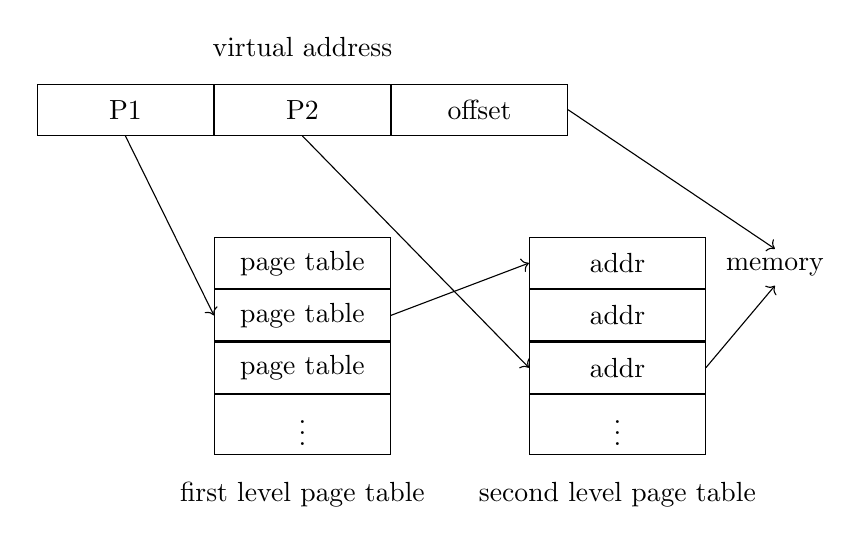
\begin{tikzpicture}
      \matrix (A) [matrix of nodes,nodes={draw, minimum size=.65cm, text width=2cm,align=center}] at (0,3)
      {
        P1 & P2 & offset \\
      };
      \matrix (T1) [matrix of nodes,nodes={draw, minimum size=.65cm, text width=2cm,align=center}] at (0,0)
      {
        page table\\
        page table\\
        page table\\
        \(\vdots\)\\
      };
      \matrix (T2) [matrix of nodes,nodes={draw, minimum size=.65cm, text width=2cm,align=center}] at (4,0)
      {
        addr\\
        addr\\
        addr\\
        \(\vdots\)\\
      };
      \node (M) at (6,1){memory};

      \draw[->] (A-1-1.south) -- (T1-2-1.west);
      \draw[->] (T1-2-1.east) -- (T2-1-1.west);
      \draw[->] (A-1-2.south) -- (T2-3-1.west);
      \draw[->] (T2-3-1.east) -- (M.south);
      \draw[->] (A-1-3.east) -- (M.north);

      \node[above=.1cm of A]{virtual address};
      \node[below=.1cm of T1]{first level page table};
      \node[below=.1cm of T2]{second level page table};
    \end{tikzpicture}

    Multilevel page tables are useful when the computer has a very large address space, giving it many pages. However, most of these usually go unused, so it represents a large saving in memory to only create page tables when they are needed.
  \end{enumerate}
\item
  \begin{enumerate}
  \item The directory service gives files a hierarchical structure and manages permissions.
  \item
    \leavevmode\vadjust{\vspace{-\baselineskip}}\newline
    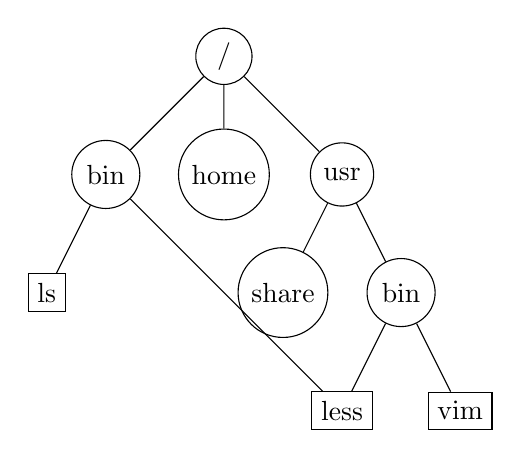
\begin{tikzpicture}
      \node[circle,draw](z){/}
      child{
        node[circle,draw](bin){bin}
        child{node[draw]{ls}}
        child[missing]{}
      }
      child{node[circle,draw]{home}}
      child{
        node[circle,draw]{usr}
        child{node[circle,draw]{share}}
        child{
          node[circle,draw]{bin}
          child{node[draw](less){less}}
          child{node[draw]{vim}}
        }
      };
      \draw (bin) -- (less);
    \end{tikzpicture}

    A directory hierarchy can be represented as a directed graph. For the convenience of garbage collection routines, it is usually required to by acyclic, which can be enforced by requiring directories to have at most one parent. In this system, the directories form a tree, but can link to non-directories arbitrarily.
  \item File metadata may store an ID or name for the file, the owner and group of the file, a count of references to the file, and dates of creation and modification.
  \item Hard linking is the way of making a file a member of a directory. A hard link is guaranteed to point to a file, and when the last hard link to a file is deleted, the space the file was using can be freed.
  \item A soft link is a file that points to another file. It is not guaranteed to point to anything, and will cause an exception if opened while not pointing to anything.
  \end{enumerate}
\item
  Unix gives each file a set of permissions. The permissions pertain separately to the owner, users in the same group as the owner, and others, and allow them to have any of read, write and execute access. More complex access control policies can be approximated by allowing files to be executed as a user other than the user who is actually using the program. The command \texttt{su} is one program offering this functionality.

  \begin{enumerate}
  \item
    \begin{tabular}{|c|c|c|c|}
      \hline
      boot block & super block & inodes & data blocks... \\
      \hline
    \end{tabular}

    The boot block is reserved for data needed in the booting process. The super block contains information about the file system, including its size and number of inodes. It also contains a pointer to a list of free data blocks. This helps with portability, since values in the super block (rather than many pieces of source code) are all that have to be changed when porting to a different file system.
  \item See question 6.
  \item With a block size of \(512\,\mathrm{B}\), 10 direct blocks, and \(4\,\mathrm{B}\) pointers, each indirect block has 128 pointers, giving a total maximum file size of \(512\,\mathrm{B}\cdot(10+128+128^2+128^3)\), which is just over \(1\,\mathrm{GiB}\).
  \item
  \end{enumerate}
\item
  It needs to be impossible for users to modify the archived files in-place, so all write permissions should be removed. However, whole archived roots should be deletable by the administrator, so (only) these directories need write permissions for the owner, with the owner being the administrator.

  It is to be noted that directories can have at most one hard link pointing to them, so in the copy process, all directories must actually be copied. However, files need not be copied until they are modified.
\item
  \begin{tabular}[t]{|l|}
    \hline
    mode (directory or regular file)\\
    \hline
    device ID, user ID, group ID\\
    \hline
    size\\
    \hline
    atime, mtime, ctime\\
    \hline
    link count\\
    \hline
    \\direct blocks\\\\
    \hline
    single indirect block\\
    \hline
    double indirect block\\
    \hline
    triple indirect block\\
    \hline
  \end{tabular}

  atime is the time of the last access to the file. mtime is the time of the last modification of the file's contents. ctime is the time of the last change of the inode or its contents. A link count (a count of hard links referencing the inode) is maintained for garbage collection. The blocks section contains an array of pointers to data blocks. Because this is of fixed size, the indirect blocks are provided. The single indirect block points to an array of pointers to data blocks, whilst the double indirect block points to an array of arrays and the triple indirect block points to an array of arrays of arrays.
\item
\item
  \begin{enumerate}
  \item There is a delay after entering an incorrect password, and passwords are never printed to the screen.
  \item The password file contains only hashes of passwords, not passwords themselves, and passwords are salted before being hashed to avoid dictionary attacks.
  \end{enumerate}
\item
  \begin{itemize}
  \item CPU
  \item Main memory
  \item Hard drive
  \item Monitor
  \item Keyboard
  \end{itemize}
\item
  \begin{enumerate}
  \item Access control lists are stored with the files they pertain to, whilst capabilities are stored with the user. With the capabilities model, it is easy to add new users with few permissions, and all such users can be given access to some shared files in an automatic way. When using ACLs, users generally have to be arranged into groups so that files can be created without needing to know exactly what users there are on the system. Deciding accessibility for capabilities is simpler, since it requires only checking a key (which can be done in hardware).
  \item
  \item
  \item Capability-based systems allow finer control of what each user can do to each file, so it is possible to get closer to the ideal of users having only the permissions they need. This improves security because it limits what users could (possibly accidentally) do, reducing the chance of the system becoming compromised.
  \end{enumerate}
\item
\end{enumerate}
\end{document}